\section{Introduction}

In Bitcoin~\cite{bitcoin}, a valid block must satisfy the
\emph{proof-of-work} inequality $H(B) < T$, where
$H$ is a hash function and $T$ is a small \emph{target}.
Simply put, valid blocks must have hashes that begin with a desired number of $0$s.
Some blocks satisfy the inequality better than others:
They have a bunch of \emph{extra} zeroes at the front of their hash.
Nevertheless, these ``heavier'' blocks are counted all the same when choosing
which chain to mine on.
We posit that the weight of a block is information
that can be useful to improve the protocol.
In this paper, we introduce \emph{\poem}.
We modify the fork choice rule of Bitcoin to take this information into account,
achieving better confirmation latency and transaction throughput.

\noindent
\myparagraph[Construction overview]
Miners still mine on the heaviest chain. We only change how chains are scored.
In Bitcoin, every block counts for the same work\footnote{Bitcoin blocks can count differently when
difficulty adjusts, but count the same during the same epoch. Our analysis is in the
static population setting~\cite{backbone}, where the population does not change with time.}.
In \poem, we give each block a score equal to the number of \emph{extra} zeroes at the front of its hash,
a value we call its \emph{intrinstic work}. Honest parties adopt the chain with the most total
intrinsic work.

\iftwocolumn
\begin{figure*}
  \centering
  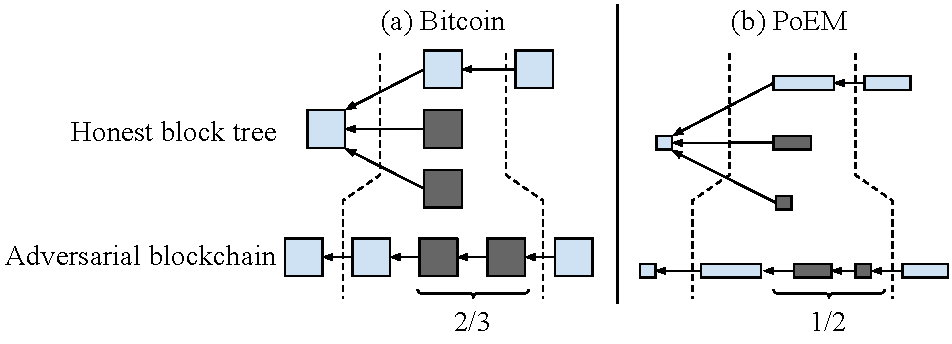
\includegraphics[width=0.6\textwidth,keepaspectratio]{figures/poem_work_wasted.pdf}
  \caption{The same block mining successes awarded to the honest parties (top) or the adversary (bottom)
           with equal mining power on Bitcoin (left) or PoEM (right) respectively. The adversary can place
           all blocks in one sequence because she does not incur any network delay. The honest parties,
           due to the delay, may place blocks at the same height (dashed section of duration $\Delta$).
           In this example, when $3$ honest blocks were found almost simultaneously, $2$ out of
           them were abandoned in Bitcoin and did not make it to the canonical longest chain
           (top-most chain).
           In the PoEM example, $2$ out of $3$ of the honest blocks were abandoned, but the cumulative intrinsic
           work wasted only happened to be $1/2$ of the intrinsic work produced during this interval.
           We illustrate the intrinsic work of a block by its size.}
  \label{fig:poem-wasted-work}
\end{figure*}
\else
\begin{figure*}
  \centering
  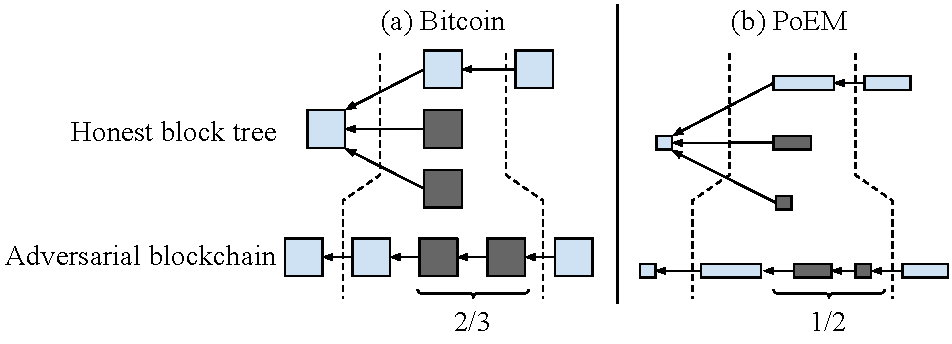
\includegraphics[width=0.8\textwidth,keepaspectratio]{figures/poem_work_wasted.pdf}
  \caption{The same block mining successes awarded to the honest parties (top) or the adversary (bottom)
           with equal mining power on Bitcoin (left) or PoEM (right) respectively. The adversary can place
           all blocks in one sequence because she does not incur any network delay. The honest parties,
           due to the delay, may place blocks at the same height (dashed section of duration $\Delta$).
           In this example, when $3$ honest blocks were found almost simultaneously, $2$ out of
           them (shaded) were abandoned in Bitcoin and did not make it to the canonical longest chain
           (top-most chain).
           In the PoEM example, $2$ out of $3$ of the honest blocks were abandoned, but the cumulative intrinsic
           work wasted only happened to be $1/2$ of the intrinsic work produced during this interval.
           In PoEM (right), we illustrate the intrinsic work of a block by its size.}
  \label{fig:poem-wasted-work}
\end{figure*}
\fi

To guarantee security, it suffices~\cite{eiar} that the work of any honest chain grows
faster than the work of the adversary's chain. Let's look at the example in Figure~\ref{fig:poem-wasted-work}.
Suppose we have three Bitcoin blocks produced in short succession.
If they were produced honestly, they will be placed in parallel.
The honest chain grows by one (Figure~\ref{fig:poem-wasted-work}, top left).

This protocol shines when blocks are produced quickly. Due to network delay, sometimes multiple honest blocks
are produced in parallel extending the same parent.
These blocks have the same height, and only one of them will
make it to the canonical chain, while the others will be discarded.
If blocks are scored equally, as in Bitcoin, the honest chain grows by one (Figure~\ref{fig:poem-wasted-work}, top left).
However, in our protocol, the heaviest block among them survives,
and the lightest blocks are discarded. The honest chain grows by the heaviest
block's score, which in expectation is more than one (Figure~\ref{fig:poem-wasted-work}, top right).

On the other hand, the adversary is mining privately independently, and placing all her blocks in sequence.
The adversary's chain growth rate is the same in PoEM and Bitcoin (Figure~\ref{fig:poem-wasted-work},
bottom left and bottom right).
This makes PoEM advantageous, since honest parties produce chains whose score grows faster
than the adversary's. Therefore, a fast PoEM configuration can be as secure as a slow Bitcoin
configuration. The resulting protocol allows for faster transaction confirmation and better
throughput while retaining the same level of security as Bitcoin.

\noindent
\myparagraph[Our contributions]
We build a protocol which retains the same level of security as Bitcoin, while achieving
better confirmation latency or transaction throughput, both because the number of confirmations
can be safely reduced and the block production rate can be safely increased.

We report on our production implementation of a real-world system
in which we employ this new rule, and show that it achieves a $28.5\%$
improvement in confirmation latency compared to Bitcoin. For this improved
latency, it also achieves a $16.3\%$ improvement in throughput.
We also theoretically prove our new protocol is secure
using the Bitcoin Backbone model. Our theoretical analysis introduces
a new technique, the \emph{real-valued random oracle}, which we prove behaves
similarly to the usual random oracle. This variant of the
random oracle allows for the use of an arsenal of theoretical tools from the
continuous domain (such as continuous distributions), easing the theoretical
exposition, and may be of independent interest.

\noindent
\myparagraph[Related work]
Bitcoin was first proven secure in the static population setting~\cite{backbone},
and later also studied in the variable population setting~\cite{varbackbone}.
The idea of using a more nuanced proof-of-work inequality in which some blocks
are considered heavier than others was first put forth by Andrew Miller~\cite{highway},
with the first complete protocol to utilize it being
Proofs of Proof-of-Work~\cite{popow}. These were later refined multiple times
to account for non\-/interactivity~\cite{nipopows}, backwards compatibility~\cite{velvet-nipopows},
onlineness~\cite{logspace}, on-chain data efficiency~\cite{compact-superblocks},
gas consumption~\cite{gasefficient-nipopows},
bribing resilience~\cite{soft-power},
and variable populations~\cite{dionyziz}.
We are the first to modify the fork choice rule to take these refinements into
account, following \ifanonymous
the
\else
our
\fi
previous short paper ``POEM: Proof of Entropy Minima''~\cite{poem-short},
where the entropic fork choice rule was defined but not analyzed.
Our work only changes the PoW inequality.
Other mechanisms refining the fork choice rule
are orthogonal and can be combined with our approach, yielding even
further performance gains.
Such examples include
PHANTOM~\cite{phantom}, SPECTRE~\cite{spectre}, GhostDAG~\cite{ghostdag}, and
GHOST~\cite{ghost}.
Additional mechanisms towards improving the latency and throughput
of proof-of-work blockchains at the consensus
layer, also composable with ours, include parallel chains~\cite{parallel-chains},
separation of transaction/consensus blocks~\cite{prism},
hybrid approaches between proof-of-work and proof-of-stake~\cite{byzcoin},
and the use of microblocks~\cite{bitcoin-ng}.